\documentclass[a4paper,10pt]{article}

\usepackage[T1]{fontenc}
\usepackage[utf8]{inputenc}
\usepackage[english]{babel}
\usepackage[skins,breakable]{tcolorbox}

\usepackage{geometry}
\geometry{
    textwidth=190mm,
    textheight=267mm,
	inner=10mm,
	outer=10mm,
	top=10mm,
	bottom=20mm
}
\usepackage{fancyhdr}
\usepackage{graphicx}
\usepackage{fontawesome}
\usepackage{hyperref}
\hypersetup{
	colorlinks = true,
	urlcolor = cyan,
	linkcolor = black,
}

%%%%%%%%%%%%%%%%%%%% - Usage Changes - %%%%%%%%%%%%%%%%%%%%
\newcommand{\professional}{Mateus Souza Oliveira}
\newcommand{\age}{26}
\newcommand{\address}{Rodovia Amaro Antônio Vieira, 2593 -- Itacorubi. Florianópolis, Santa Catarina, Brazil}
\newcommand{\phone}{+55 (48) 9 9810-2694}
\newcommand{\email}{matews1943@gmail.com}
\renewcommand{\date}{\today}
\newcommand{\about}{
    Proactive, detailed, determined and always seeking to improve myself. Currently, I am working as a web developer. I have experience with Python, Git, Docker, SQL, Linux, JavaScript, Tests, Code Quality tools, Continuous Integration, PostgreSQL and GitHub, GitLab and Bitbucket. I am fluent in English.\\

    I am interested in working with Python and automation. I prefer to work on Linux.
	\vspace{\baselineskip}
}
%%%%%%%%%%%%%%%%% - End of Usage Changes - %%%%%%%%%%%%%%%%

\setlength{\fboxrule}{2pt}
\setlength{\fboxsep}{0pt}

\fancyhead{} % Header: reset
\fancyfoot{} % Footer: reset
\fancyfoot[C]{Page \thepage \ of \pageref{lastPage}} % Footer: center
\fancyfoot[R]{Made with \LaTeX} % Footer: right
\fancyfoot[L]{Updated in \date} % Footer: left
\renewcommand{\headrulewidth}{0pt} % Header line thickness
\renewcommand{\footrulewidth}{0.4pt} % Footer line thickness
\pagestyle{fancy} % Sets the page style

\newcommand{\createSection}[4][0]{
	\begin{tcolorbox}[
        blanker,
        breakable,
        title=\begin{minipage}{0.16\linewidth}\large{\textbf{#2}}\vspace{-#3\baselineskip}\end{minipage},
        coltitle=black,
        leftupper=0.21\linewidth,
    ]
        #4
		\ifnum0#1>0 { \hrule {\ } } \fi
    \end{tcolorbox}
}

\begin{document}

	\noindent
	\fbox{
	\hspace*{-3.35\fboxrule}
	\begin{minipage}{0.3\linewidth}
		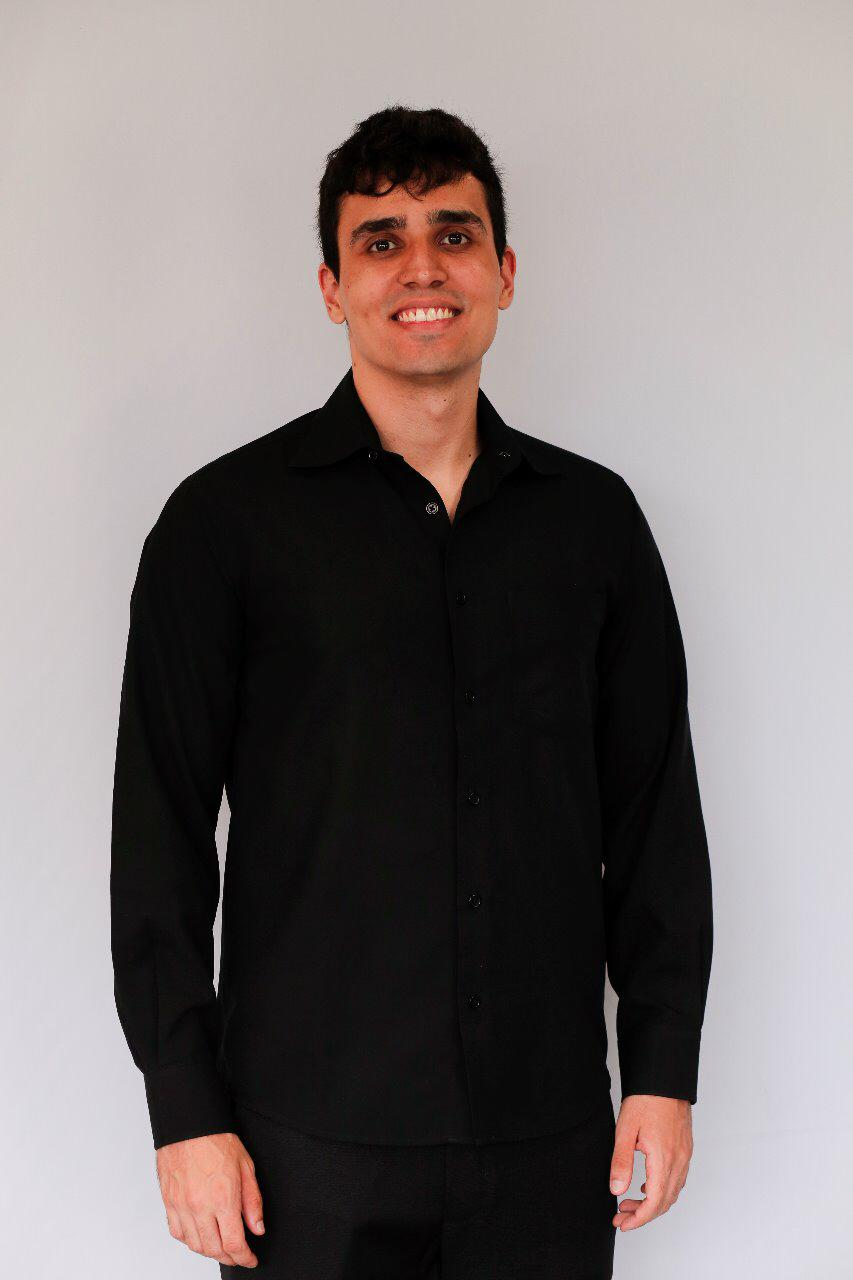
\includegraphics[width=\linewidth]{img/profile.jpeg}
	\end{minipage}
	\hspace*{-3.35\fboxrule}
	}
	\hfill
	\begin{minipage}{0.65\linewidth}
		\Huge{\bf \professional, \age}\\\vspace{-1.75\baselineskip}

		\noindent\rule{\textwidth}{1.5pt} {\ }\\\vspace{-1.8\baselineskip}

		\large{
		\faMapMarker \ \address \\
		\begin{minipage}{0.5\linewidth}
			\faWhatsapp \ \phone
		\end{minipage}
		\begin{minipage}{0.5\linewidth}
			\faEnvelope \ \email
		\end{minipage}
		\begin{minipage}{0.5\linewidth}
			\faLinkedinSquare \ \href{https://www.linkedin.com/in/mateusoliveira43/}{\texttt{/mateusoliveira43}}
		\end{minipage}
		\begin{minipage}{0.5\linewidth}
			\faGithub \ \href{https://github.com/mateusoliveira43}{\texttt{/mateusoliveira43}}
		\end{minipage}
		\faLink \ \href{https://mateusoliveira43.github.io/}{\texttt{mateusoliveira43.github.io}}\\
		\vfill
		\textbf{About}:\about
		}
	\end{minipage}
	\vspace{\baselineskip}

%%%%%%%%%%%%%%%%%%%%%% - CV's Body - %%%%%%%%%%%%%%%%%%%%%%
    \createSection[1]{Education}{2}{
		\textit{Mathematics - Bachelor Degree}, Federal University of Santa Catarina (UFSC), Florianópolis, Santa Catarina \hfill 2014 - 2020 \\
	}

	\createSection[1]{Experience}{2}{
	    \textit{Junior Software Developer}, Fundação CERTI, Florianópolis, Santa Catarina \hfill October 2020 - currently \\
	    March 2022 - Currently\\
        \textbf{Activities}: Updating the internal site of Fundação CERTI.\\

        October 2020 - February 2022\\
        \textbf{Activities}: WEB project and desktop application (beyond translation of calculations code in Visual Basic to Python), from national company, involving Python (PyPy, FastAPI, SQLAlchemy, Numpy, Pandas) in the Backend, JavaScript (TypeScript, Node.js, React) in the Frontend, PostgreSQL in the database. All the code being continuous integrated by Jenkins, having quality measures by tests, linter and SonarQube and containerized with Docker.\\

        Acting in the creation of structure of the site's frontend, definition of the database's structure (along the client and mechanical/petroleum engineer team), revisions and implementations (both in the backend and in the frontend) and automation. Beyond that, I was one of the leaders of the team (which consisted with development, QA, UX and mechanical/petroleum engineer squads). Planning and working following some of the agile methodologies principles.\\

        August 2021 - January 2022\\
        \textbf{Activities}: Legacy Linux embedded project with WEB interface (HMI), from German company, involving C++ in the device, JavaScript (Meteor) in the Backend and Frontend, SQLite in the database. Code being continuous integrated by GitLab, having quality measures by tests, linter and containerized with Docker.\\

        Acting in the implementation of improvements of the continuous integration of the repositories and automation improvements with Python. Planning and working in English.\\

	    \textit{Scientific Initiation Scholarship}, Federal University of Santa Catarina (UFSC), Florianópolis, Santa Catarina \hfill August 2019 - February 2020 \\
		\textbf{Activities}: Research focused in Computer Graphics.\\

		\textit{Laboratory of Mathematical and Technological Studies (LEMAT) Scholarship}, Federal University of Santa Catarina (UFSC), Florianópolis, Santa Catarina \hfill March 2019 - July 2019 \\
		\textbf{Activities}: Application, development and update of project files.\\

		\textit{Regional Mathematical Olympiad of Santa Catarina (ORM) Journal Scholarship}, Federal University of Santa Catarina (UFSC), Florianópolis, Santa Catarina \hfill March 2016 - March 2017 \\
		\textbf{Activities}: Application and development of training files; correction and development of test files; update of journal master file.\\

		\textit{Tutorial Education Program in Mathematics (PET Matemática) Scholarship}, Federal University of Santa Catarina (UFSC), Florianópolis, Santa Catarina \hfill March 2015 - February 2016 \\
		\textbf{Activities}: Application and development of training files; teaching in pre-university preparatory course; teaching and elaboration of \LaTeX\ and Matlab mini courses.\\
	}

    \createSection[1]{Programming languages and tools}{4}{
        \large{\bf
			\begin{minipage}{0.65\linewidth}
				Python (FastAPI, pytest, unittest, argparse)\\
				JavaScript (TypeScript, Node.js, React, Jest)\\
				Docker (Docker Compose)\\
				Linux\\
				GitHub\\
				Bitbucket\\
				PostgreSQL\\
			\end{minipage}
			\begin{minipage}{0.35\linewidth}
				Git\\
				SQL\\
				HTML\\
				CSS (Bootstrap)\\
				GitLab\\
				Jenkins\\
				\vspace{\baselineskip}
			\end{minipage}
		}
    }

	\createSection{Languages}{2}{
	    \large{
			\begin{minipage}{0.5\linewidth}
				\textbf{Portuguese}: native \\
				\textbf{English}: fluent \\
				\textbf{French}: basic \\
			\end{minipage}
			\begin{minipage}{0.5\linewidth}
				\textbf{Spanish}: basic \\
				\textbf{German}: basic \\
				\vspace{\baselineskip}
			\end{minipage}
		}
	}
%%%%%%%%%%%%%%%%%%% - End of CV's Body - %%%%%%%%%%%%%%%%%%
    \label{lastPage}
\end{document}
